\documentclass{beamer}
\setbeamercovered{transparent}
\usepackage{listings}
\usepackage[T1]{fontenc}
\usepackage{booktabs}

\usetheme[pageofpages=of,% String used between the current page and the
                         % total page count.
          bullet=circle,% Use circles instead of squares for bullets.
          titleline=true,% Show a line below the frame title.
          titlepagelogo=opensuse,
          alternativetitlepage=true,% Use the fancy title page.
          ]{Torino}


% Define some styles
\lstdefinestyle{mybash}{
  language=bash,
  basicstyle=\footnotesize\ttfamily,
  keywordstyle=\color{blue}\ttfamily,
  stringstyle=\color{red}\ttfamily,
  commentstyle=\color{green}\ttfamily,
  morecomment=[l][\color{magenta}]{\#}
}

\lstdefinestyle{myperl}{
  language=Perl,
  basicstyle=\footnotesize\ttfamily,
  keywordstyle=\color{blue}\ttfamily,
  stringstyle=\color{red}\ttfamily,
  commentstyle=\color{green}\ttfamily,
  morecomment=[l][\color{magenta}]{\#}
}

\lstdefinestyle{mypython}{
  language=Python,
  showstringspaces=false,
  basicstyle=\footnotesize\ttfamily,
  keywordstyle=\color{blue}\ttfamily,
  stringstyle=\color{red}\ttfamily,
  commentstyle=\color{green}\ttfamily,
  morecomment=[l][\color{magenta}]{\#}
}


% Counter commands for enumerates
\newcounter{saveenumi}
\newcommand{\seti}{\setcounter{saveenumi}{\value{enumi}}}
\newcommand{\conti}{\setcounter{enumi}{\value{saveenumi}}}


\setbeamerfont{title}{series=\bfseries,size=\LARGE}
\author{Alberto Planas <aplanas@suse.de>\newline {\small openSUSE Team}}
\title{How to write OBS plugins -- oSC14}
\subtitle{Extend the functionality of OBS}


\AtBeginSection[]{
  \setbeamercolor{background canvas}{bg=chameleongreen3}
  \begin{frame}[plain]
    \begin{center}\begin{huge}\textcolor{white}{\secname}\end{huge}\end{center}
  \end{frame}
  \setbeamercolor{background canvas}{bg=}
}

\AtBeginSubsection[]{
  \setbeamercolor{background canvas}{bg=chameleongreen3}
  \begin{frame}[plain]
    \begin{center}\begin{huge}\textcolor{white}{\subsecname}\end{huge}\end{center}
  \end{frame}
  \setbeamercolor{background canvas}{bg=}
}


\begin{document}

\begin{frame}[t,plain]
  \titlepage
\end{frame}


\section{Introduction}

\begin{frame}{OBS Architecture Overview}
  \begin{figure}
    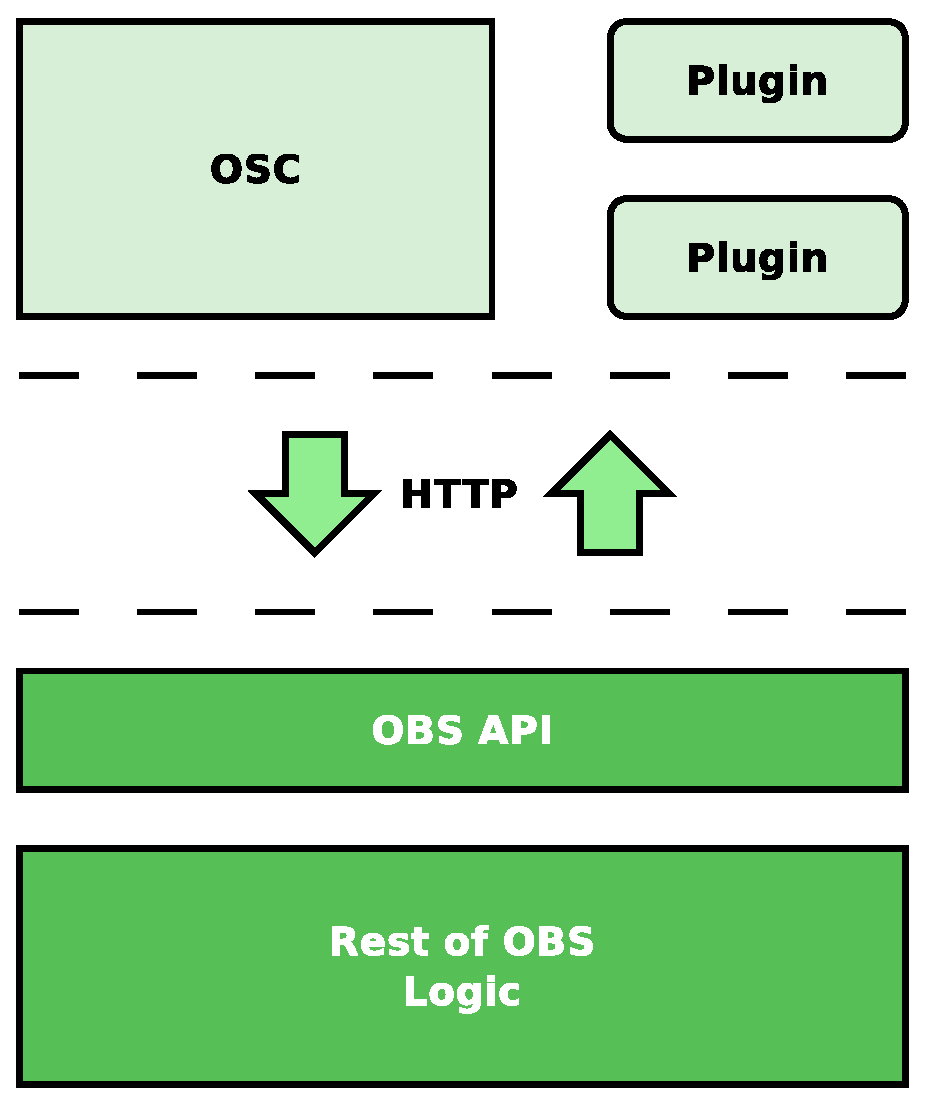
\includegraphics[width=5.5cm]{obsplugins.eps}
  \end{figure}
\end{frame}

\begin{frame}{OSC and OBS Relation}
  \begin{itemize}
  \item OSC is an interface to OBS
  \item Can be extended using plugins
  \item Use HTTP request to the API, using a REST-like protocol
  \item Results are usually serialized in XML
  \item And is written in Python!
  \end{itemize}
\end{frame}


\section{A Basic Example}

\begin{frame}[fragile]
  \frametitle{First Example. Print Raw Request}
  \lstset{style=mypython}
  \begin{lstlisting}
from osc import cmdln
from osc.core import http_GET
from osc.core import makeurl

@cmdln.alias('vr')
def do_viewrequest(self, subcmd, opts, *args):
    """${cmd_name}: view the raw content of a request

    Usage:
       ${cmd_name} SR ...
           View the raw content of a request
    ${cmd_option_list}
    """
    apiurl = self.get_api_url()
    for sr in args:
        url = makeurl(apiurl, ['request', str(sr)])
        print http_GET(url).read()
  \end{lstlisting}
\end{frame}

\begin{frame}[fragile]
  \frametitle{Pluging Deployment}
  \lstset{style=mypython}
  \begin{lstlisting}
    # Copy or create a link
    ln -sr example1.py ~/.osc-plugins

    # Check that the new command is there
    osc --help

    # Check that docstring is OK
    osc vr --help
  \end{lstlisting}
\end{frame}

\begin{frame}{OSC Plugins}
  An OSC plugin consist in:
  \begin{itemize}
  \item An entry point (do\_XXX) as a unbounded method
  \item A function decorator to set parameters and alias
  \item A docstring to describe the command, with examples
  \item A way to create request to OBS API (GET and POST)
  \item We can use high level functions from osc.core
  \item A way to parse XML results
  \end{itemize}
\end{frame}

\begin{frame}[fragile]
  \frametitle{Plugin Entry Point}
  \begin{itemize}
  \item The entry point is an unbounded method for the class osc.Osc
  \item This allows you to access some functions via self
  \item You decorate the function (method) with @cmdln to add parameters:
    \lstset{style=mypython}
    \begin{lstlisting}
      @cmdln.alias('vr')
      @cmdln.option('-p', '--project', action='append', help='project')
    \end{lstlisting}
    Use the same syntax that Python optparse library
  \item The docstring will appear when {\em osc command --help}
  \end{itemize}
\end{frame}

\begin{frame}[fragile]
  \frametitle{Low Level Functions}
  In {\em osc.core} you can find some low level functions to access OBS API. 
  \begin{itemize}
  \item {\em makeurl()} -- Build the URL needed to access a service
  \item {\em http\_[GET|POST|PUT|DELETE]()} -- To create a HTTP request to the URL
  \item {\em ET.parse()} -- Use cElementTree to parse the XML
  \end{itemize}
  \lstset{style=mypython}
  \begin{lstlisting}
    url = makeurl(apiurl, [<PATH>], query=<QUERY_DIC>)
    try:
        root = ET.parse(http_GET(url)).getroot()
    except urllib2.HTTPError, e:
        print('ERROR in URL %s [%s]' % (url, e))
  \end{lstlisting}
\end{frame}

\begin{frame}[fragile]
  \frametitle{Examples of URLs. Change review status}
  \lstset{style=mypython}
  \begin{lstlisting}
# Use POST to change the review status of a request
query = {
  'cmd': 'changereviewstate',
  'newstate': 'declined'
  'by_user': 'the_boos',
}
url = makeurl(opts.apiurl, ['request', sr_id], query=query)
try:
  root = ET.parse(http_POST(url, data='Sorry')).getroot()
  code = root.attrib['code']
except urllib2.HTTPError, e:
  print('ERROR in URL %s [%s]' % (url, e))
  \end{lstlisting}
\end{frame}

\begin{frame}[fragile]
  \frametitle{Examples of URLs. User information}
  \lstset{style=mypython}
  \begin{lstlisting}
# Get user information
url = makeurl(apiurl, ['person', 'aplanas'])
try:
  root = ET.parse(http_GET(url)).getroot()
  print root.find("realname").text, root.find("email").text
except urllib2.HTTPError, e:
  print('ERROR in URL %s [%s]' % (url, e))
  \end{lstlisting}
\end{frame}

\begin{frame}[fragile]
  \frametitle{High Level Functions}
  Dig into {\em osc.core} to find more high level functions
  \begin{lstlisting}
    # Print user's email
    from osc.core import get_user_data
    get_user_data(apiurl, u, 'email')

    # Search packages
    from osc.core import search
    xpath = "@name='%s' or @name='%s'" % (pkg1, pkg2)
    result = search(apiurl, package=xpath)
  \end{lstlisting}
\end{frame}

\section{A Full Example: Foo}
%% Show here a demo of foo.py code. Or skip if you do not have time

\begin{frame}{I Want to Learn More}
  \begin{itemize}
  \item An introduction about OSC plugins\newline
    {\small\url{http://en.opensuse.org/openSUSE:OSC_plugins}}
  \item OSC Collab. An excellent plugin from the GNOME team\newline
    {\small\url{https://en.opensuse.org/openSUSE:Osc_Collab}}
    {\small\url{https://github.com/openSUSE/osc-plugin-collab}}
  \item The Repo Checker pluging. Now with Staging\newline
    {\small\url{https://github.com/openSUSE/osc-plugin-factory}}
  \end{itemize}
\end{frame}

\section{End Note}

\begin{frame}{SUSE is hiring}
  \begin{figure}
    
\includegraphics[width= 0.8\linewidth]{suse_hiring.png}
  \end{figure}
\end{frame}

\begin{frame}{Thanks}
  \begin{center}
    Thank you for your attention.
  \end{center}
\end{frame}

\end{document}
